\section{Theoretical (scientific/technological background)}
\subsection{Main Theoretical Concepts / Terminologies}
\subsubsection{Computer Vision}	
Computer Vision (CV) is a field of Artificial Intelligence that enables computers to see and interpret the real world.
In any given image, the machine will only receive a NumPy Array containing values (0-255) that represent the light intensity of each pixel, without a way to understand the information, it can't perceive objects the way humans can.
However, by providing it with structured data, algorithms can be trained to identify color and pixel patterns, allowing them to accurately classify objects~\cite{sas_computervision, kumari2025hand}.

\subsubsection{Color Space}	
A Color Space is a mathematical model that defines how the colors are represented numerically in an image, each pixel stores a value or a set of values that instruct the screen on what light intensities to emit, depending on the model, these numerical values will represent very different colors.
\newline

\textbf{RGB (Red Green Blue)} - 
The Default Format used by most Deep Learning Models and the standard for every Phone or TV screen, Monitor or LED, each pixel consists of 3 smaller sub-pixels, Red, Green, and Blue, by varying the light intensity of each sub-pixel (0-255), the system can display any given color~\cite{roboflow_colorspaces}.

\begin{table}[h]
\centering
\renewcommand{\arraystretch}{1.2} 
\begin{tabular}{|c|c|c|l|}
\hline
\textbf{Red (R)} & \textbf{Green (G)} & \textbf{Blue (B)} & \textbf{Color Name} \\ \hline
0                & 0                  & 0                  & Black               \\ \hline
255              & 255                & 255                & White               \\ \hline
255              & 0                  & 0                  & Red                 \\ \hline
0                & 255                & 0                  & Green               \\ \hline
0                & 0                  & 255                & Blue                \\ \hline
0                & 255                & 255                & Cyan                \\ \hline
255              & 0                  & 255                & Magenta             \\ \hline
255              & 128                & 0                  & Orange              \\ \hline
\end{tabular}
\caption{Examples of RGB Color Values}
\label{tab:rgb_values}
\end{table}

\textbf{BGR (Blue Green Red)} - 
The Default Format used by the OpenCV Library, due to it being developed in 1999 when the BGR color format was the standard for software development and camera manufacturers~\cite{mallick_bgr}. In essence, it is similar to the RGB Format, with the notable difference of the Red and Blue channels swapped, in order to implement a Deep Learning Model with OpenCV, it's required to manually convert the image to the standard RGB format.

\vspace{0.3cm}
\textbf{HSV (Hue Saturation Value)} - 
While RGB is what hardware uses to display color, the HSV format aligns more closely to how people perceive color, it consists of 3 different values:
\newline Hue - The base color represented on a 360º color wheel
\newline Saturation - Intensity of the color, from vibrant to faded
\newline Brightness Value - Amount of light is hitting the color
\newline Because the Hue component remains consistent regardless of lighting variations, this format is ideal for projects that require object tracking and color segmentation~\cite{roboflow_colorspaces, mopidevi2023hand}.

\begin{figure}[h]
    \centering  
    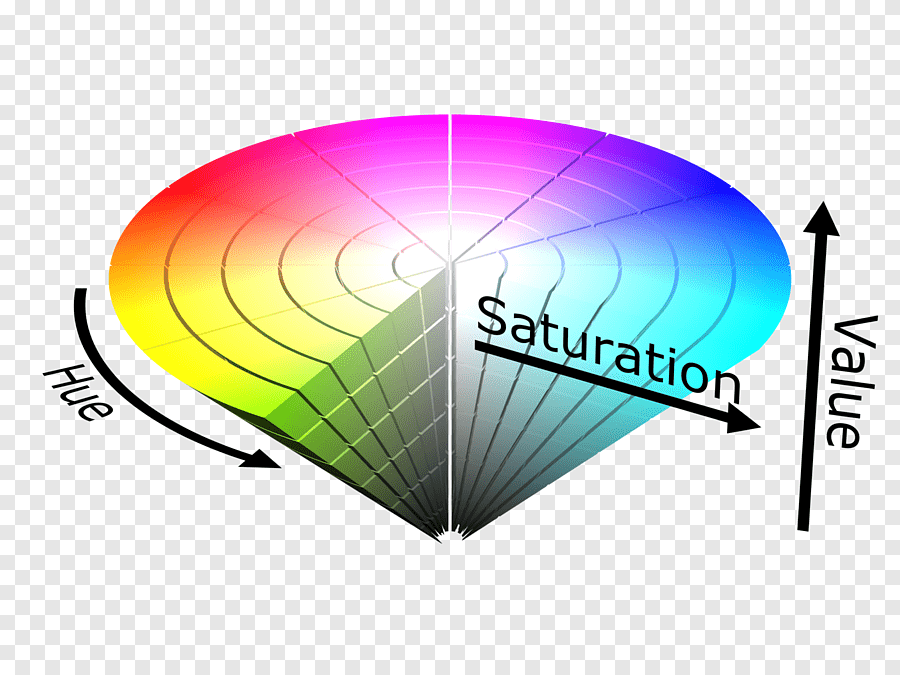
\includegraphics[width=0.5\textwidth]{imagens/HSV.png} 
    \caption{HSV Color Pattern} 
\end{figure}

\newpage
\textbf{Grayscale} - 
Grayscale is a single-channel image format that removes all hue and saturation, leaving only its brightness value, by reducing the three channels down to only one~\cite{deep2025intellimotion}, it greatly decreases the processing load, and its increased simplicity enables the creation of color masks that can filter out backgrounds and simplify complex objects for easier analysis, this is a fundamental pre-processing step for Algorithm and Deep Learning training.

\begin{figure}[h]
    \centering 
    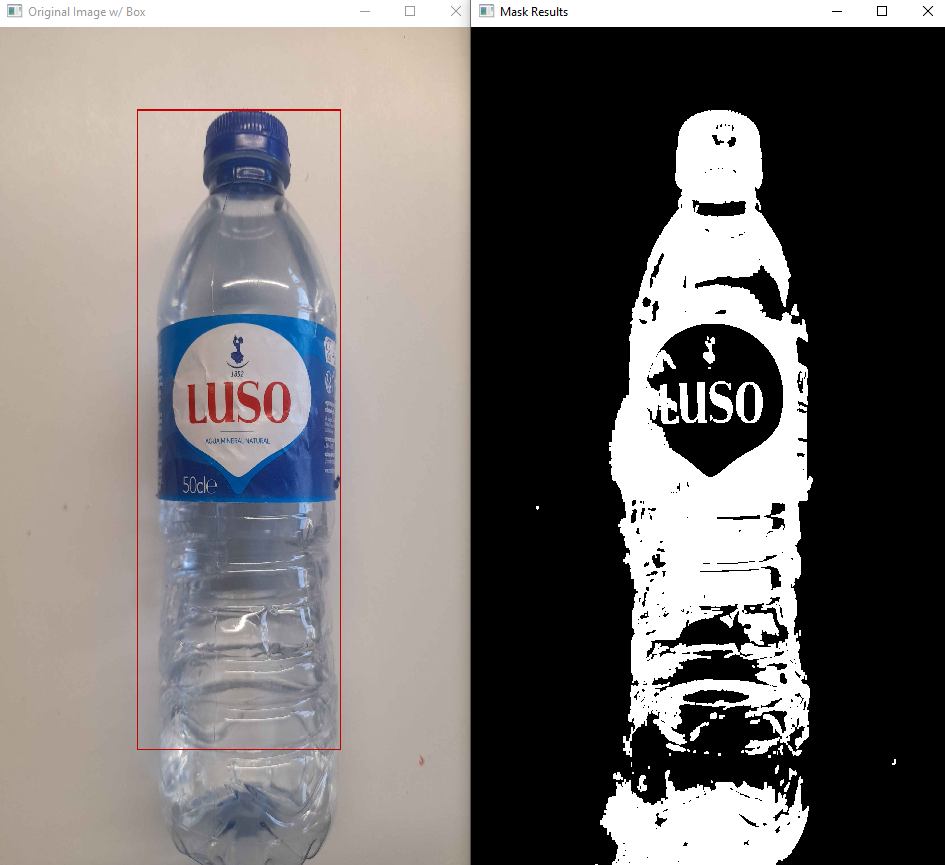
\includegraphics[width=0.5\textwidth]{imagens/Color Mask Example.png} 
    \caption{Color Mask Example using Grayscale} 
\end{figure}

\subsubsection{Inference}
Inference is the process where an AI Algorithm makes predictions based on the data provided, in this project, the data consists of the live feed being captured by the camera, which is continuously being fed into the model for analysis, because of the nature of this software, the inference must be done with relatively high speed and precision to ensure low latency and smooth operation.

\subsubsection{Landmarks}
The last step of the analysis is show its results, once Inference is done correctly, the model will return 21 sets of coordinates (x,y,z), these are landmarks spread throughout the hand, from the wrist to the finger tips, the software then reconstructs the hand gesture by connecting these coordinates together, creating a uniform pattern that will allow us to use a model and recognize what motion or gesture the hand is making.

\subsection{State-of-the-Art}

\subsubsection{VSCode \& Python}
VSCode is a lightweight but versatile Integrated Development Environment (IDE) with support for hundreds of languages. Python is one of the most widely used programming languages, known for its versatility, fast prototyping, and beginner friendly, it was chosen for having better integration with OpenCV and MediaPipe, and being able to perform complex mathematical operations while maintaining a fast performance.

\subsubsection{OpenCV}
OpenCV is an Open Source Computer Vision Library that acts as the eyes for this project, as well as the bridge between the camera feed and the software, it's responsible for the frame acquisition, its pre-processing, the drawing of the model inference results, as well as displaying the softwares' logic directly onto the video feed, the library has more than 2500 algorithms and it's a versatile tool that works efficiently with other AI Models for a wide range of computer vision projects, from object detection to face recognition, this tool was chosen for its ease-of-use, optimized real-time performance and image processing~\cite{opencv_about}.
	
\subsubsection{MediaPipe Model}
MediaPipe is an open source framework developed by Google, it specializes in real time, machine learning solutions for live video, audio and streaming~\cite{mediapipe_main}, for this project it uses an Inference engine for hand tracking, it uses a palm detector and a landmark model to draw 21 points throughout the image of a hand with very low latency~\cite{mediapipe_hands}, which enables it to work in tandem with the camera and OpenCV to continuously analyze the images and display the results at a very high speed~\cite{deep2025intellimotion}.